Fig. \ref{fig:sigma} below shows the of $\sigma$ on $J^{*}$ with $\sigma$.\\
\begin{figure}[!h]
	\caption{Evolution of $J^{*}$ with $\sigma$}
	\label{fig:sigma}
	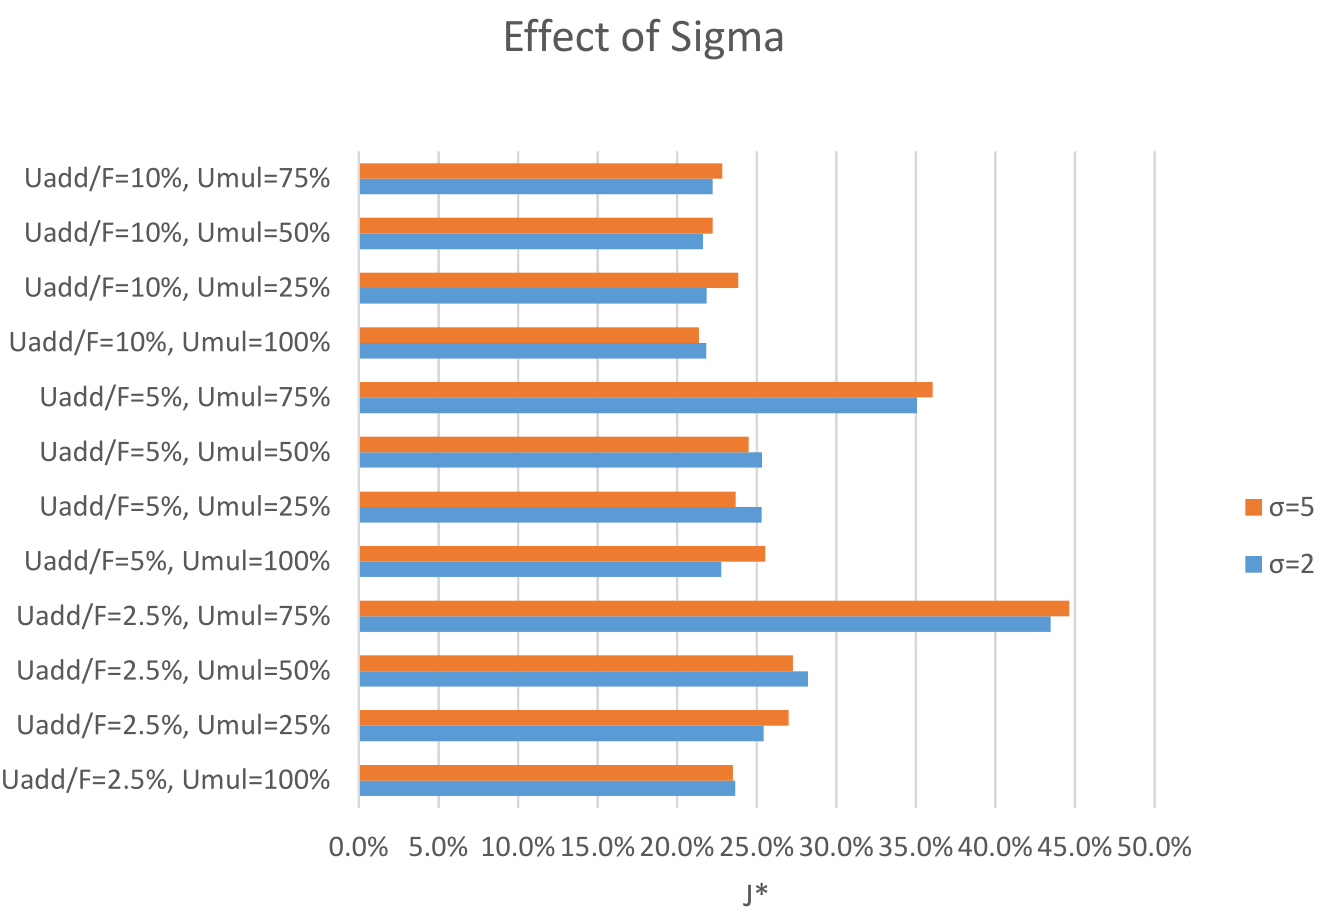
\includegraphics[width=7in]{figures/sigma.png}
\end{figure}\\
$\sigma$ has no influence on $J^{*}$ in our case. That is because of the small search space dimension and because, due to the inexact templates shapes, many knob configurations give the same result quality (i.e. there are many equivalent (almost) global minima).\\
\\
As observed in the figures of \ref{subsec:umul} and \ref{subsec:uadd}, increasing $\sigma$ makes the initial  "very messy part" of the knobs convergence to be larger (up to 1000 iterations instead of 500). However, once the knobs start converging, they are more likely to stay around the same value until the end of the execution if $\sigma$ is larger. This is illustrated in Fig. \ref{fig:umulknobs100}, where the comparison between the two plots of the last column shows that the knobs do not converge with $\sigma=2$ while they do with $\sigma=5$.\\
In addition, we observe in Fig. \ref{fig:umulcp75} that the strange congestion shapes are avoided if $\sigma=5$, but this could be fortuitous.\\
\\
\emph{Conclusion:} In our case, $\sigma \in [2,5]$ for [0-10] scaled knobs has almost no influence. There is a slight preference for $\sigma=5$ in a few cases. \\
$\sigma$ will probably have a greater importance if the dimension of the search space is bigger i.e. there are more knobs; or if the templates have better shapes, allowing for greater quality results i.e. fewer equivalent global minima.